\documentclass[sigconf]{acmart}
\usepackage[utf8]{inputenc}
\usepackage{booktabs} % For formal tables
\usepackage{balance} % For balanced columns on the last page

\copyrightyear{2019} 
\acmYear{2019} 
\setcopyright{acmcopyright}
\acmConference[MobileApps 2019]{Building Web and Mobile Apps 2019}{Winter term 2018/2019}{Fulda, Germany}
\acmBooktitle{MobileApps 2019: Building Web and Mobile Apps 2019, winter term 2018/2019, Fulda, Germany}
\acmPrice{0.00}
%\acmDOI{0}
%\acmISBN{0}

% Use the "authoryear" citation style, and make sure citations are in [square brackets].
\citestyle{acmauthoryear}
\setcitestyle{square}

% A useful command for controlling the number of authors per row.
% The default value of "authorsperrow" is 2.
\settopmatter{authorsperrow=0}

% end of preamble.

\begin{document}

% Title. 
% If your title is long, consider \title[short title]{full title} - "short title" will be used for running heads.
\title[Unity Mobile Games]{Improving the performance of Unity mobile games}

% Authors.
\author{Dan-Andrei Iorga 1154111}
\affiliation{
  \institution{Fulda University of Applied Sciences}
  \streetaddress{Leipziger Stra{\ss}e 123}
  \postcode{36037} 
  \city{Fulda} 
  \country{Germany}
}
\email{dan-andrei.iorga@informatik.hs-fulda.de}


% This command defines the author string for running heads.
\renewcommand{\shortauthors}{A. Iorga}

% abstract
\begin{abstract}
Game engines such as Unity are convenient ways to center the development process on the game behaviour itself rather than hardware-level implementations. While they are powerful tools that can increase the productivity of the developers, this comes at the cost of efficiency. Ways must be devised to mitigate the performance loss of a premade engine to acceptable results. This paper will present the study of a sample game implemented in Unity and the results of applying various perfromance-improving techniques on it.
\end{abstract}

%
% The code below should be generated by the tool at
% http://dl.acm.org/ccs.cfm
% Please copy and paste the code below.
%

\keywords{
	Unity, 
	Game engines, 
	Games, 
	Mobile Applications,
	Mobile Games,
	Android, 
	Game development, 
	Application performance
}


% A "teaser" figure, centered below the title and authors and above the body of the work.
\begin{teaserfigure}
  \centering
  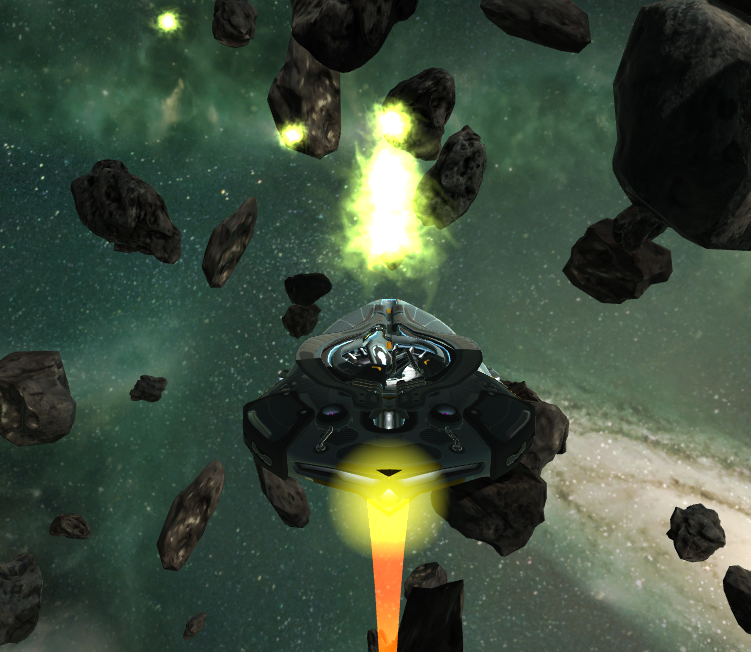
\includegraphics[width=\linewidth]{images/teaser}
  \caption{Space Shooter screenshot}
  \label{fig:teaser}
  \vspace{0.03cm}
\end{teaserfigure}
% Processes all of the front-end information and starts the body of the work.
\maketitle
\section{Introduction}
\subsection{Components of a game}
\subsection{Games vs Hardware}
\subsection{Space Shooter}
Lorem ipsum dolor sit amet, consectetur adipiscing elit. Vestibulum nisl ante, commodo non ligula non, ultrices mollis ante. Mauris dignissim justo a nibh vestibulum consectetur. Aenean sollicitudin, turpis ac fringilla cursus, nulla quam scelerisque est, at blandit ex felis in urna. Fusce in quam eleifend odio dignissim mollis. Aliquam eleifend lectus massa, ac vestibulum tellus ullamcorper eget. Proin lacus eros, tempor ac elementum a, tempus eu urna. Vestibulum vitae eros ac nulla placerat elementum nec sed tortor. Sed in urna metus. Praesent quis nisl nisi. Duis pharetra risus sed bibendum molestie. Aliquam nunc augue, finibus a diam ac, dignissim porttitor est.
Lorem ipsum dolor sit amet, consectetur adipiscing elit. Vestibulum nisl ante, commodo non ligula non, ultrices mollis ante. Mauris dignissim justo a nibh vestibulum consectetur. Aenean sollicitudin, turpis ac fringilla cursus, nulla quam scelerisque est, at blandit ex felis in urna. Fusce in quam eleifend odio dignissim mollis. Aliquam eleifend lectus massa, ac vestibulum tellus ullamcorper eget. Proin lacus eros, tempor ac elementum a, tempus eu urna. Vestibulum vitae eros ac nulla placerat elementum nec sed tortor. Sed in urna metus. Praesent quis nisl nisi. Duis pharetra risus sed bibendum molestie. Aliquam nunc augue, finibus a diam ac, dignissim porttitor est.
Lorem ipsum dolor sit amet, consectetur adipiscing elit. Vestibulum nisl ante, commodo non ligula non, ultrices mollis ante. Mauris dignissim justo a nibh vestibulum consectetur. Aenean sollicitudin, turpis ac fringilla cursus, nulla quam scelerisque est, at blandit ex felis in urna. Fusce in quam eleifend odio dignissim mollis. Aliquam eleifend lectus massa, ac vestibulum tellus ullamcorper eget. Proin lacus eros, tempor ac elementum a, tempus eu urna. Vestibulum vitae eros ac nulla placerat elementum nec sed tortor. Sed in urna metus. Praesent quis nisl nisi. Duis pharetra risus sed bibendum molestie. Aliquam nunc augue, finibus a diam ac, dignissim porttitor est.
Lorem ipsum dolor sit amet, consectetur adipiscing elit. Vestibulum nisl ante, commodo non ligula non, ultrices mollis ante. Mauris dignissim justo a nibh vestibulum consectetur. Aenean sollicitudin, turpis ac fringilla cursus, nulla quam scelerisque est, at blandit ex felis in urna. Fusce in quam eleifend odio dignissim mollis. Aliquam eleifend lectus massa, ac vestibulum tellus ullamcorper eget. Proin lacus eros, tempor ac elementum a, tempus eu urna. Vestibulum vitae eros ac nulla placerat elementum nec sed tortor. Sed in urna metus. Praesent quis nisl nisi. Duis pharetra risus sed bibendum molestie. Aliquam nunc augue, finibus a diam ac, dignissim porttitor est.
\subsection{Performance testing}
Lorem ipsum dolor sit amet, consectetur adipiscing elit. Vestibulum nisl ante, commodo non ligula non, ultrices mollis ante. Mauris dignissim justo a nibh vestibulum consectetur. Aenean sollicitudin, turpis ac fringilla cursus, nulla quam scelerisque est, at blandit ex felis in urna. Fusce in quam eleifend odio dignissim mollis. Aliquam eleifend lectus massa, ac vestibulum tellus ullamcorper eget. Proin lacus eros, tempor ac elementum a, tempus eu urna. Vestibulum vitae eros ac nulla placerat elementum nec sed tortor. Sed in urna metus. Praesent quis nisl nisi. Duis pharetra risus sed bibendum molestie. Aliquam nunc augue, finibus a diam ac, dignissim porttitor est.
Lorem ipsum dolor sit amet, consectetur adipiscing elit. Vestibulum nisl ante, commodo non ligula non, ultrices mollis ante. Mauris dignissim justo a nibh vestibulum consectetur. Aenean sollicitudin, turpis ac fringilla cursus, nulla quam scelerisque est, at blandit ex felis in urna. Fusce in quam eleifend odio dignissim mollis. Aliquam eleifend lectus massa, ac vestibulum tellus ullamcorper eget. Proin lacus eros, tempor ac elementum a, tempus eu urna. Vestibulum vitae eros ac nulla placerat elementum nec sed tortor. Sed in urna metus. Praesent quis nisl nisi. Duis pharetra risus sed bibendum molestie. Aliquam nunc augue, finibus a diam ac, dignissim porttitor est.
Lorem ipsum dolor sit amet, consectetur adipiscing elit. 
\begin{figure}[bhp]

\includegraphics[width=\columnwidth]{images/radeonrtx}
\end{figure}
Vestibulum nisl ante, commodo non ligula non, ultrices mollis ante. Mauris dignissim justo a nibh vestibulum consectetur. Aenean sollicitudin, turpis ac fringilla cursus, nulla quam scelerisque est, at blandit ex felis in urna. Fusce in quam eleifend odio dignissim mollis. Aliquam eleifend lectus massa, ac vestibulum tellus ullamcorper eget. Proin lacus eros, tempor ac elementum a, tempus eu urna. Vestibulum vitae eros ac nulla placerat elementum nec sed tortor. Sed in urna metus. Praesent quis nisl nisi. Duis pharetra risus sed bibendum molestie. Aliquam nunc augue, finibus a diam ac, dignissim porttitor est.
Lorem ipsum dolor sit amet, consectetur adipiscing elit. Vestibulum nisl ante, commodo non ligula non, ultrices mollis ante. Mauris dignissim justo a nibh vestibulum consectetur. Aenean sollicitudin, turpis ac fringilla cursus, nulla quam scelerisque est, at blandit ex felis in urna. Fusce in quam eleifend odio dignissim mollis. Aliquam eleifend lectus massa, ac vestibulum tellus ullamcorper eget. Proin lacus eros, tempor ac elementum a, tempus eu urna. Vestibulum vitae eros ac nulla placerat elementum nec sed tortor. Sed in urna metus. Praesent quis nisl nisi. Duis pharetra risus sed bibendum molestie. Aliquam nunc augue, finibus a diam ac, dignissim porttitor est.
\subsection{Improving performance}
Lorem ipsum dolor sit amet, consectetur adipiscing elit. Vestibulum nisl ante, commodo non ligula non, ultrices mollis ante. Mauris dignissim justo a nibh vestibulum consectetur. Aenean sollicitudin, turpis ac fringilla cursus, nulla quam scelerisque est, at blandit ex felis in urna. Fusce in quam eleifend odio dignissim mollis. Aliquam eleifend lectus massa, ac vestibulum tellus ullamcorper eget. Proin lacus eros, tempor ac elementum a, tempus eu urna. Vestibulum vitae eros ac nulla placerat elementum nec sed tortor. Sed in urna metus. Praesent quis nisl nisi. Duis pharetra risus sed bibendum molestie. Aliquam nunc augue, finibus a diam ac, dignissim porttitor est.
Lorem ipsum dolor sit amet, consectetur adipiscing elit. Vestibulum nisl ante, commodo non ligula non, ultrices mollis ante. Mauris dignissim justo a nibh vestibulum consectetur. Aenean sollicitudin, turpis ac fringilla cursus, nulla quam scelerisque est, at blandit ex felis in urna. Fusce in quam eleifend odio dignissim mollis. Aliquam eleifend lectus massa, ac vestibulum tellus ullamcorper eget. Proin lacus eros, tempor ac elementum a, tempus eu urna. Vestibulum vitae eros ac nulla placerat elementum nec sed tortor. Sed in urna metus. Praesent quis nisl nisi. Duis pharetra risus sed bibendum molestie. Aliquam nunc augue, finibus a diam ac, dignissim porttitor est.
Lorem ipsum dolor sit amet, consectetur adipiscing elit. Vestibulum nisl ante, commodo non ligula non, ultrices mollis ante. Mauris dignissim justo a nibh vestibulum consectetur. Aenean sollicitudin, turpis ac fringilla cursus, nulla quam scelerisque est, at blandit ex felis in urna. Fusce in quam eleifend odio dignissim mollis. Aliquam eleifend lectus massa, ac vestibulum tellus ullamcorper eget. Proin lacus eros, tempor ac elementum a, tempus eu urna. Vestibulum vitae eros ac nulla placerat elementum nec sed tortor. Sed in urna metus. Praesent quis nisl nisi. Duis pharetra risus sed bibendum molestie. Aliquam nunc augue, finibus a diam ac, dignissim porttitor est.
Lorem ipsum dolor sit amet, consectetur adipiscing elit. Vestibulum nisl ante, commodo non ligula non, ultrices mollis ante. Mauris dignissim justo a nibh vestibulum consectetur. Aenean sollicitudin, turpis ac fringilla cursus, nulla quam scelerisque est, at blandit ex felis in urna. Fusce in quam eleifend odio dignissim mollis. Aliquam eleifend lectus massa, ac vestibulum tellus ullamcorper eget. Proin lacus eros, tempor ac elementum a, tempus eu urna. Vestibulum vitae eros ac nulla placerat elementum nec sed tortor. Sed in urna metus. Praesent quis nisl nisi. Duis pharetra risus sed bibendum molestie. Aliquam nunc augue, finibus a diam ac, dignissim porttitor est.
\subsection{Object pooling}
Lorem ipsum dolor sit amet, consectetur adipiscing elit. Vestibulum nisl ante, commodo non ligula non, ultrices mollis ante. Mauris dignissim justo a nibh vestibulum consectetur. Aenean sollicitudin, turpis ac fringilla cursus, nulla quam scelerisque est, at blandit ex felis in urna. Fusce in quam eleifend odio dignissim mollis. Aliquam eleifend lectus massa, ac vestibulum tellus ullamcorper eget. Proin lacus eros, tempor ac elementum a, tempus eu urna. Vestibulum vitae eros ac nulla placerat elementum nec sed tortor. Sed in urna metus. Praesent quis nisl nisi. Duis pharetra risus sed bibendum molestie. Aliquam nunc augue, finibus a diam ac, dignissim porttitor est.
Lorem ipsum dolor sit amet, consectetur adipiscing elit. Vestibulum nisl ante, commodo non ligula non, ultrices mollis ante. Mauris dignissim justo a nibh vestibulum consectetur. Aenean sollicitudin, turpis ac fringilla cursus, nulla quam scelerisque est, at blandit ex felis in urna. Fusce in quam eleifend odio dignissim mollis. Aliquam eleifend lectus massa, ac vestibulum tellus ullamcorper eget. Proin lacus eros, tempor ac elementum a, tempus eu urna. Vestibulum vitae eros ac nulla placerat elementum nec sed tortor. Sed in urna metus. Praesent quis nisl nisi. Duis pharetra risus sed bibendum molestie. Aliquam nunc augue, finibus a diam ac, dignissim porttitor est.
Lorem ipsum dolor sit amet, consectetur adipiscing elit. Vestibulum nisl ante, commodo non ligula non, ultrices mollis ante. Mauris dignissim justo a nibh vestibulum consectetur. Aenean sollicitudin, turpis ac fringilla cursus, nulla quam scelerisque est, at blandit ex felis in urna. Fusce in quam eleifend odio dignissim mollis. Aliquam eleifend lectus massa, ac vestibulum tellus ullamcorper eget. Proin lacus eros, tempor ac elementum a, tempus eu urna. Vestibulum vitae eros ac nulla placerat elementum nec sed tortor. Sed in urna metus. Praesent quis nisl nisi. Duis pharetra risus sed bibendum molestie. Aliquam nunc augue, finibus a diam ac, dignissim porttitor est.
Lorem ipsum dolor sit amet, consectetur adipiscing elit. Vestibulum nisl ante, commodo non ligula non, ultrices mollis ante. Mauris dignissim justo a nibh vestibulum consectetur. Aenean sollicitudin, turpis ac fringilla cursus, nulla quam scelerisque est, at blandit ex felis in urna. Fusce in quam eleifend odio dignissim mollis. Aliquam eleifend lectus massa, ac vestibulum tellus ullamcorper eget. Proin lacus eros, tempor ac elementum a, tempus eu urna. Vestibulum vitae eros ac nulla placerat elementum nec sed tortor. Sed in urna metus. Praesent quis nisl nisi. Duis pharetra risus sed bibendum molestie. Aliquam nunc augue, finibus a diam ac, dignissim porttitor est.
\subsection{Texture resolution}
Lorem ipsum dolor sit amet, consectetur adipiscing elit. Vestibulum nisl ante, commodo non ligula non, ultrices mollis ante. Mauris dignissim justo a nibh vestibulum consectetur. Aenean sollicitudin, turpis ac fringilla cursus, nulla quam scelerisque est, at blandit ex felis in urna. Fusce in quam eleifend odio dignissim mollis. Aliquam eleifend lectus massa, ac vestibulum tellus ullamcorper eget. Proin lacus eros, tempor ac elementum a, tempus eu urna. Vestibulum vitae eros ac nulla placerat elementum nec sed tortor. Sed in urna metus. Praesent quis nisl nisi. Duis pharetra risus sed bibendum molestie. Aliquam nunc augue, finibus a diam ac, dignissim porttitor est.
Lorem ipsum dolor sit amet, consectetur adipiscing elit. Vestibulum nisl ante, commodo non ligula non, ultrices mollis ante. Mauris dignissim justo a nibh vestibulum consectetur. Aenean sollicitudin, turpis ac fringilla cursus, nulla quam scelerisque est, at blandit ex felis in urna. Fusce in quam eleifend odio dignissim mollis. Aliquam eleifend lectus massa, ac vestibulum tellus ullamcorper eget. Proin lacus eros, tempor ac elementum a, tempus eu urna. Vestibulum vitae eros ac nulla placerat elementum nec sed tortor. Sed in urna metus. Praesent quis nisl nisi. Duis pharetra risus sed bibendum molestie. Aliquam nunc augue, finibus a diam ac, dignissim porttitor est.
Lorem ipsum dolor sit amet, consectetur adipiscing elit. Vestibulum nisl ante, commodo non ligula non, ultrices mollis ante. Mauris dignissim justo a nibh vestibulum consectetur. Aenean sollicitudin, turpis ac fringilla cursus, nulla quam scelerisque est, at blandit ex felis in urna. Fusce in quam eleifend odio dignissim mollis. Aliquam eleifend lectus massa, ac vestibulum tellus ullamcorper eget. Proin lacus eros, tempor ac elementum a, tempus eu urna. Vestibulum vitae eros ac nulla placerat elementum nec sed tortor. Sed in urna metus. Praesent quis nisl nisi. Duis pharetra risus sed bibendum molestie. Aliquam nunc augue, finibus a diam ac, dignissim porttitor est.
Lorem ipsum dolor sit amet, consectetur adipiscing elit. Vestibulum nisl ante, commodo non ligula non, ultrices mollis ante. Mauris dignissim justo a nibh vestibulum consectetur. Aenean sollicitudin, turpis ac fringilla cursus, nulla quam scelerisque est, at blandit ex felis in urna. Fusce in quam eleifend odio dignissim mollis. Aliquam eleifend lectus massa, ac vestibulum tellus ullamcorper eget. Proin lacus eros, tempor ac elementum a, tempus eu urna. Vestibulum vitae eros ac nulla placerat elementum nec sed tortor. Sed in urna metus. Praesent quis nisl nisi. Duis pharetra risus sed bibendum molestie. Aliquam nunc augue, finibus a diam ac, dignissim porttitor est.
\subsection{Object managers}
Lorem ipsum dolor sit amet, consectetur adipiscing elit. Vestibulum nisl ante, commodo non ligula non, ultrices mollis ante. Mauris dignissim justo a nibh vestibulum consectetur. Aenean sollicitudin, turpis ac fringilla cursus, nulla quam scelerisque est, at blandit ex felis in urna. Fusce in quam eleifend odio dignissim mollis. Aliquam eleifend lectus massa, ac vestibulum tellus ullamcorper eget. Proin lacus eros, tempor ac elementum a, tempus eu urna. Vestibulum vitae eros ac nulla placerat elementum nec sed tortor. Sed in urna metus. Praesent quis nisl nisi. Duis pharetra risus sed bibendum molestie. Aliquam nunc augue, finibus a diam ac, dignissim porttitor est.
Lorem ipsum dolor sit amet, consectetur adipiscing elit. Vestibulum nisl ante, commodo non ligula non, ultrices mollis ante. Mauris dignissim justo a nibh vestibulum consectetur. Aenean sollicitudin, turpis ac fringilla cursus, nulla quam scelerisque est, at blandit ex felis in urna. Fusce in quam eleifend odio dignissim mollis. Aliquam eleifend lectus massa, ac vestibulum tellus ullamcorper eget. Proin lacus eros, tempor ac elementum a, tempus eu urna. Vestibulum vitae eros ac nulla placerat elementum nec sed tortor. Sed in urna metus. Praesent quis nisl nisi. Duis pharetra risus sed bibendum molestie. Aliquam nunc augue, finibus a diam ac, dignissim porttitor est.
Lorem ipsum dolor sit amet, consectetur adipiscing elit. Vestibulum nisl ante, commodo non ligula non, ultrices mollis ante. Mauris dignissim justo a nibh vestibulum consectetur. Aenean sollicitudin, turpis ac fringilla cursus, nulla quam scelerisque est, at blandit ex felis in urna. Fusce in quam eleifend odio dignissim mollis. Aliquam eleifend lectus massa, ac vestibulum tellus ullamcorper eget. Proin lacus eros, tempor ac elementum a, tempus eu urna. Vestibulum vitae eros ac nulla placerat elementum nec sed tortor. Sed in urna metus. Praesent quis nisl nisi. Duis pharetra risus sed bibendum molestie. Aliquam nunc augue, finibus a diam ac, dignissim porttitor est.
Lorem ipsum dolor sit amet, consectetur adipiscing elit. Vestibulum nisl ante, commodo non ligula non, ultrices mollis ante. Mauris dignissim justo a nibh vestibulum consectetur. Aenean sollicitudin, turpis ac fringilla cursus, nulla quam scelerisque est, at blandit ex felis in urna. Fusce in quam eleifend odio dignissim mollis. Aliquam eleifend lectus massa, ac vestibulum tellus ullamcorper eget. Proin lacus eros, tempor ac elementum a, tempus eu urna. Vestibulum vitae eros ac nulla placerat elementum nec sed tortor. Sed in urna metus. Praesent quis nisl nisi. Duis pharetra risus sed bibendum molestie. Aliquam nunc augue, finibus a diam ac, dignissim porttitor est.
\section{Conclusions}
XXX Some example text with cites: 
Frameworks like Apple ARKit \cite{ARKit} and Google ARCore \cite{ARCore} provide an easy use of
computer vision based tracking technologies to build new mobile Augmented Reality applications.
XXX Especially in the automotive industry mobile AR-based training and infotainment apps, like 
the "Mobile Augmented Reality Technical Assistance" project described in \cite{Stanimirovic14}, 
are becoming more and more a selling point. Therefore, XXX
%\input{chapters/relatedwork}
%\input{chapters/concept}
%\input{chapters/implementation}
%\input{chapters/results}
%In this paper we have looked at several means of improving and stabilizing the performance of a sample game implemented in Unity. While the end results may not be called extreme, significant improvements can be seen between the initial and final reading as per table 5. Looking again at the first and last values, using a few basic techniques, Space Shooter has gained more than doubled the average framerate on PC with extremely similar deviations, and the Android version was improved by over 91\%, albeit with more fluctuations. \\
Looking at the rest of the entries, we can see that the previous statements hold true, with extremely similar changes between the original and optimized version of the game.
``The one constant cost included in all performance optimization work is time. So, with
limited time at our disposal to both implement the features we want to implement and keep
everything working, an important skill to learn for any developer is workflow optimization.
Better understanding of the tools we use will save us more time in the long run, and
hopefully provide the extra time we need to implement everything we want to, which
applies not only to the Unity Engine, but to every tool we use.''\cite{optimizationbook}
\begin{table}
\caption{Optimization data}
\label{tab:conf}
\begin{minipage}{0.49\textwidth}
\begin{center}
\begin{tabular}{lllll}
Value & PC pre & PC post & Android pre & Android post \\
Mean & 75.00 & 155.04 & 10.30 & 19.70 \\
Std & 2.51 & 2.77 & 0.67 & 7.12 \\
Top 10 mean & 76.00 & 159.20 & 12.30 & 28.60 \\
Bottom 10 mean & 67.50 & 150.30 & 10.00 & 10.00 \\
Min & 62 & 146 & 10 & 10 \\
Max & 76 & 160 & 13 & 29 
\end{tabular}
\bigskip
\end{center} 
\end{minipage}
\end{table}
\begin{acks}
This work was carried out within the Web and Mobile Apps class.
\end{acks}

\bibliographystyle{ACM-Reference-Format}
\bibliography{literature}

\end{document}
